\documentclass[11pt, a4paper]{article}
\usepackage[french]{babel}
\usepackage{amsmath}
\usepackage{amsfonts}   % if you want the fonts
\usepackage{amssymb}    % if you want extra symbols
\usepackage{graphicx}  % need for figures
\usepackage{geometry}
\usepackage{tocloft}
\usepackage{secdot}
\sectiondot{section}
\sectiondot{subsection}
\renewcommand{\cftsecaftersnum}{.}
\renewcommand{\cftsubsecaftersnum}{.}		
\usepackage[utf8]{inputenc}
\usepackage{ragged2e}
\usepackage[hidelinks]{hyperref}

\begin{document}	
\begin{titlepage}
\centering
\LARGE{\textsc{Analyse et classification d'urls à des fins de segmentation automatique par groupes de ciblage}}\\
\vfill
\large Matthieu Brito Antunes\\
\large Data Scientist\\
\large Tradelab - Paris\\
\large septembre 2020\\
\end{titlepage}

\newpage
\tableofcontents
\listoftables
\listoffigures
\thispagestyle{empty}

\newpage
\pagenumbering{arabic}

\section{Introduction}
\label{sec:intro}

L'ensemble des adresses web (URL) des pages visitées sur Internet peut constituer une source pertinente lorsque l'on souhaite réfléchir à une méthode de ciblage publicitaire. Les informations extraites à partir du traitement des URL permettent de comprendre les mécanismes qui régissent le regroupement d'utilisateurs, ou \textit{segmentation}. 

La segmentation d'utilisateurs est une étape cruciale dans le processus de ciblage publicitaire en ligne et peut s'avérer très chronophage. Il apparaît donc essentiel de chercher à utiliser toute information qui permettrait de comprendre comment tendre vers son automatisation totale.

Les informations contenues dans la structure des URL nous renseignent principalement sur l'organisation globale d'un site web, et la manière dont sont créées les URL associées aux nouvelles pages. Ceci permet de construire des regroupements de pages web sans avoir à analyser leur contenu. Ces regroupements pourraient idéalement être réalisés de manière automatique, à partir d'un modèle de \textit{clustering} qui recevrait une URL en entrée et fournirait en sortie le groupe auquel elle appartient après avoir analysé sa structure.

Ce rapport présente le travail de construction d'un modèle d'analyse et de classification automatique d'URL. La première partie du rapport est centrée sur l'étude de la problématique et des enjeux associés. Diverses pistes d'analyse de structure d'URL sont proposées. La seconde partie du rapport offre une vision théorique de la solution proposée pour automatiser la création de segments à partir des données d'URL collectées chaque jour chez Jellyfish France. La dernière partie du rapport présente la mise en place de la solution et les résultats obtenus sur des données récoltées sur une période fixe.

\section{Segmentation d'URL}

Le nombre croissant de visites de pages web et de liens échangés constitue un défi auquel doivent faire face les ingénieurs et chercheurs appliqués dans le vaste domaine du \textit{web mining}. L'analyse de l'information contenue dans les pages web et les renseignements que des séquences d'URL peuvent apporter sont cruciaux lorsqu'il s'agit de mettre en place des stratégies visant à optimiser l'utilisation d'Internet, que ce soit à des fins publicitaires (ciblage, analyse de parcours de navigation), de sécurité (détection d'URL de pages malveillantes), de construction de moteurs de recherche, pour l'archivage du web, etc.

\section{Analyse de la structure des URL et premiers essais de segmentation automatique via \textit{pattern trees}}

\subsection{Structure classique d'une URL}

Sur Internet, les pages web regroupent divers formats de données (texte, image, son...) et sont repérées par une chaîne de caractères renseignant deux choses :
\begin{itemize}
	\item leur emplacement
	\item le protocole internet permettant d'y accéder\footnote{Les protocoles les plus connus sont ceux que l'on rencontre tous les jours dans la barre d'adresse de notre navigateur : \texttt{http} et \texttt{https} pour \textit{HyperText Transfer Protocol (Secure)}.}
\end{itemize}

Cette chaîne de caractères, appelée \textit{adresse web} ou encore URL (pour \textit{Uniform Resource Locator}) est générée pour chaque nouvelle page ajoutée à un site, et permet donc à l'utilisateur de savoir où il se trouve. Encore faut-il qu'il sache la lire ! On retrouve en effet plusieurs éléments constitutifs d'une URL, qui peuvent être présent ou absents selon le type de site sur lequel l'utilisateur se trouve. Globalement, une URL peut être décrite comme suit :

\begin{center}

\texttt{http://www.bing.com/images/search?q=hp\&form=bifd}

\end{center}

avec 

\begin{itemize}
	\item \texttt{http} : \textit{scheme} 
	\item \texttt{www.bing.com} : \textit{authority}
	\item \texttt{images/search} : \textit{path}
	\item \texttt{q=hp\&form=bifd} : \textit{query}
\end{itemize}

\subsection{Analyse de la structure des URLs via \textit{pattern trees}}

La première approche vise à mettre en évidence des structures caractéristiques au sein des URL en faisant appel à des outils analogues aux arbres de décision~\cite{lei}. L'idée est ici d'apprendre à transformer des URL doublons en une forme canonique à l'aide de règles de réécriture. A partir des règles d'écriture dégagées après analyse des URL disponibles, la segmentation automatique est possible sur de nouvelles URL, en considérant que les URL soumises aux mêmes règles de réécriture appartiennent au même segment.

L'ensemble des règles de réécriture est regroupé dans un \textit{pattern tree}, i.e. un groupe de structures d'URL organisé selon une certaine hiérarchie. Au sein de cet arbre, chaque nœud représente un groupe d'URL ayant la même structure syntaxique. Cet arbre permet de rassembler l'ensemble de l'information statistique relative aux URL à disposition, augmentant ainsi la robustesse et la fiabilité du processus de segmentation.
 C'est sur cette idée que la première approche de ce travail est basée pour essayer de créer automatiquement des segments d'URL présentant des similitudes sans avoir à analyser le contenu des pages auxquelles elles renvoient (fig.~\ref{pattern_tree}).

\begin{figure}[!h]
	\center
	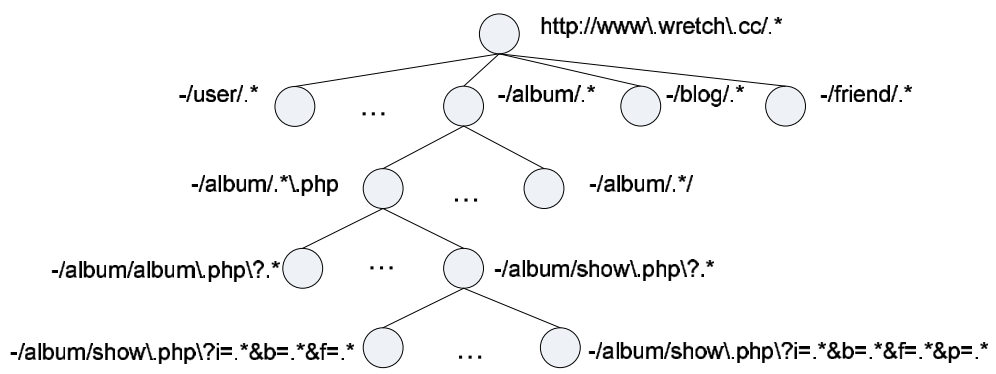
\includegraphics[scale=0.6]{pattern_tree.png}
	\caption{Exemple de \textit{pattern tree} construit à partir du site \texttt{www.wretch.cc}}
	\label{pattern_tree}
\end{figure}

\subsection{Résultats de transformations d'URL et orientation vers une autre méthode}

L'utilisation d'un \textit{pattern tree} pour regrouper des URL en se basant sur leurs similarités syntaxiques présente l'inconvénient d'être principalement adaptée aux URL d'un seul et même site web. Lorsque l'algorithme de construction du \textit{pattern tree} est fourni en URL trop différentes les unes des autres, des résultats peu significatifs peuvent être observés, le principal (et le plus fâcheux) étant l'obtention d'un unique segment d'URL transformées en la forme \texttt{http://*/*/*}. On s'aperçoit qu'au sein de ce segment toutes les URL sont regroupées et qu'il ne présente par conséquent aucune spécificité exploitable dans l'optique d'un ciblage publicitaire d'utilisateurs.

\section{Approche statistique de la classification automatique d'URL}

La seconde approche adoptée s'est basée sur des outils largement répandus dans le domaine des systèmes de recommandation et d'analyse des préférences d'utilisateurs~\cite{morichetta}. Le principe de cette approche statistique est basé sur le calcul de distance entre les objets à classer. D'une façon générale, retenons que tout objet que l'on cherche à faire passer par un processus de classification automatique (ou segmentation) peut être représenté par un vecteur. En d'autres termes, il est possible de projeter les caractéristiques des objets que l'on cherche à classifier dans un espace au sein duquel leur classification est possible à l'aide de techniques de calcul efficaces.

\subsection{Distance et similarité}

En mathématiques, l'idée de distance renvoie à une application bien particulière visant à quantifier la \textit{similarité} entre deux points $x_1$ et $x_2$ du plan ou de l'espace. Une mesure de similarité est appelée \textit{distance} si et seulement si elle respecte les propriétés suivantes :

\begin{itemize}
	\item $d(x_1, x_2) \geq 0, d(x_1, x_2) = 0 \iff x_1 = x_2$ (positivité)
	\item $d(x_1, x_2) = d(x_2, x_1)$ (symmétrie)
	\item $d(x_1, x_3) \leq d(x_1, x_2) + d(x_2, x_3) \forall (x_1, x_2, x_3)$ (inégalité triangulaire)
\end{itemize}

Il existe plusieurs manières de calculer la distance entre deux objets. On utilise l'une d'elles dans la vie de tous les jours sans même s'en apercevoir dans les espaces à deux ou trois dimensions : la distance Euclidienne, définie par la racine de la somme des différences entre les coordonnées des deux objets élevées au carré\footnote{Pour deux objets $x = (x_1, x_2, \dots, x_n)$ et $y = (y_1, y_2, \dots, y_n)$, la distance qui les sépare vaut $\sqrt{\sum_{i=1}^n (x_i-y_i)^2}$}.

Ici, la distance utilisée tient compte du fait que les objets à classer ne sont plus de simples points dans l'espace, mais des URL, qui sont en somme des chaînes de caractères. Trois mesures de distance entre deux URL $s_1$ et $s_2$ ont été étudiées : la distance de Levenshtein\footnote{$d_{\text{LVS}} = \begin{cases}
  \max(i,j) & \text{ if } \min(i,j)=0, \\
  \min \begin{cases}
          d_{\text{LVS}}(i-1,j) + 1 \\
          d_{\text{LVS}}(i,j-1) + 1 \\
          d_{\text{LVS}}(i-1,j-1) + 1_{(a_i \neq b_j)}
       \end{cases} & \text{ otherwise.}
\end{cases}$}, la distance de Jaro\footnote{$d_{\text{Jaro}} = \frac{1}{3}\left(\frac{m}{|s_1|} + \frac{m}{|s_2|} + \frac{m-t}{m}\right)$ où $|s_i|$ est la longueur de la chaîne de caractères $s_i$, $m$ est le nombre de ''caractères correspondants'' et $t$ est le nombre de ''transpositions''}, et une version modifiée de la distance de Levenshtein\footnote{$d_{\text{URL} (s_1, s_2)} = 1 - \frac{|s_1| + |s_2| - d_{\text{LVS2}}(s_1, s_2)}{|s_1| + |s_2|}$ où $d_{\text{LVS2}}$ est une modification de $d_{\text{LVS}}$ pondérant les remplacements de caractères par 2 plutôt que par 1}.

Pour ce travail, la dernière mesure de distance $d_{\text{URL}}$ a été retenue.

\subsection{DBSCAN et segmentation}

Une fois la distance entre chaque objet mesurée, il faut constituer automatiquement des groupes au sein desquels celle-ci n'excède pas une valeur seuil choisie avec parcimonie. Si cette valeur seuil est trop élevée, les groupes risquent de se révéler trop grands, englobant ainsi trop d'hétérogénéité. Si elle est au contraire trop petite, les groupes risquent de ne pas capturer assez d'information, et de trop nombreux groupes risquent d'être créés. 

Tout ce processus de construction de groupes porte en apprentissage statistique le nom de \textit{clustering}, et peut être réalisé au moyen de méthodes diverses et variées. Ici, c'est la méthode DBSCAN\footnote{\textit{Density-Based Spatial Clustering of Applications with Noise} est un algorithme utilisant la distance entre deux points et le nombre minimum de points choisis pour constituer un \textit{cluster} comme paramètres de segmentation automatique} qui a été choisie, par souci d'efficacité et de rapidité d'exécution.

Rappelons que l'idée derrière le \textit{clustering} est de créer des groupes d'objets homogènes suffisamment denses pour contenir assez d'information, et suffisamment distincts pour que cette information soit correctement distribuée. DBSCAN fonctionne sur le principe suivant : $\epsilon$ est le rayon dans lequel doivent se trouver au moins $MinPts$ points ou plus pour que soit constituée un \textit{cluster}. Pour un nouveau point donné, l'algorithme vérifie par la suite que son $\epsilon$-voisinage contient au moins $MinPts$ points. Ce nouveau point appartient donc alors à un nouveau \textit{cluster}, et l'$\epsilon$-voisinage est parcouru de proche en proche afin de définir les limites de ce \textit{cluster}.

\subsection{Résultats et limitations de la méthode}

Une étape essentielle dans ce genre de travaux consiste à observer l'influence de la variation des paramètres des algorithmes que l'on utilise sur les résultats obtenus, c'est la \textit{sensitivity analysis}. Ici, les deux paramètres que l'on peut faire varier touchent directement à la taille des \textit{clusters} créés par DBSCAN, il s'agit du rayon $\epsilon$ et du nombre de points minimum $MinPoints$ les constituant.

Dans les faits, nous avons obtenu des résultats significatifs et exploitables. Même si l'analyse aurait pu être poussée plus loin, nous nous satisfaisons pour l'instant des résultats que nous avons. On observe une claire variation du nombre de \textit{clusters} créés et de la proportion de points considérés comme du bruit\footnote{Donc pas intégrés à un \textit{cluster}} en fonction du rayon $\epsilon$ de \textit{clustering} utilisé (fig.~\ref{clustering})

\begin{figure}[!h]
	\center
	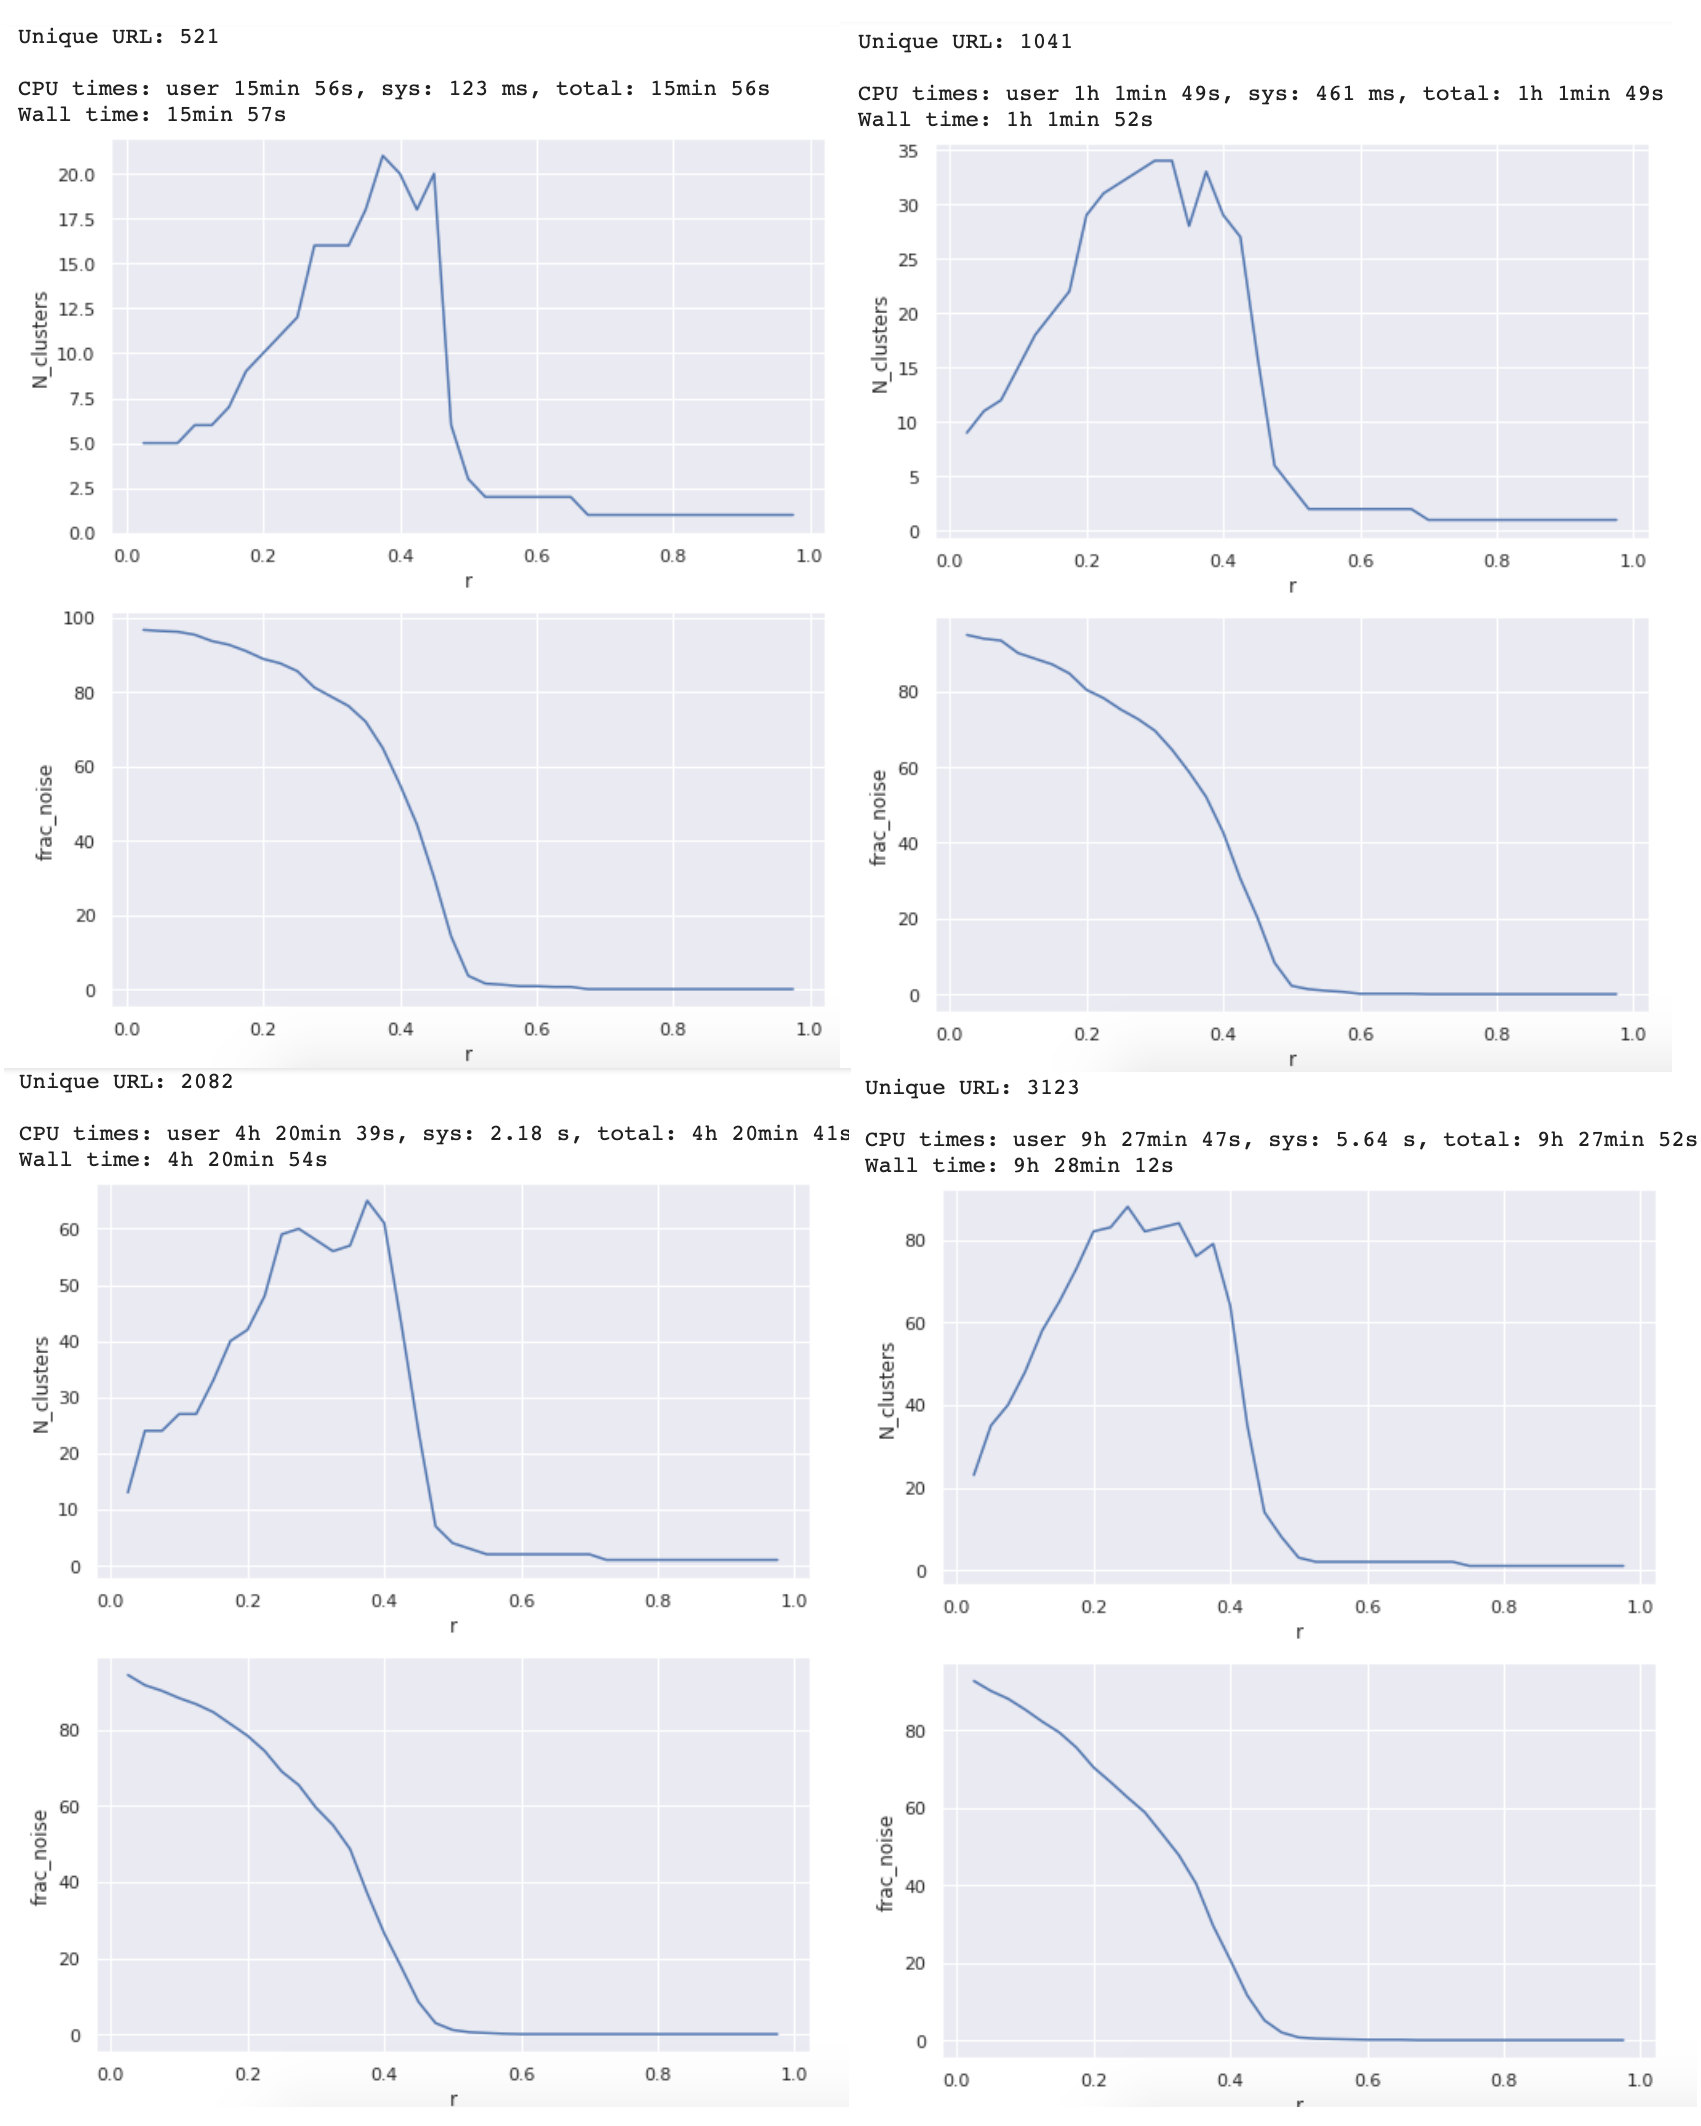
\includegraphics[scale=0.1]{clustering.png}
	\caption{Résultats de \textit{clustering} par DBSCAN selon différentes valeurs de $\epsilon$ et $MinPoints$}
	\label{clustering}
\end{figure}

\section{Approche sémantique de l'analyse des URL et segmentation automatique par la méthode des \textit{n}-grammes}

La dernière approche a fait appel à un concept développé pour le traitement de problématiques liées à la théorie de l'information. Ici, l'idée est de classer automatiquement les URL (de créer des segments) sans avoir à les décortiquer ou à les diviser en leurs caractères constitutifs. Le modèle $n$-grammes s'est révélé plutôt bien adapté.

\subsection{Le modèle $n$-grammes}

D'une manière générale, un $n$-gramme est une séquence de $n$ éléments construite à partir d'une séquence donnée~\cite{abdallah}. On se donne un ensemble de documents $D = \{d_1, d_2, \dots, d_n\}$ et un ensemble de classes auxquelles on cherche à assigner chaque document $C = \{c_1, c_2, \dots, c_k\}$. Pour un document $d_i$, la probabilité $p(c_j|d_i)$ qu'il appartienne à la classe $c_j$ peut s'exprimer à l'aide du théorème de Bayes par :

\[
p(c_j|d_i) = \frac{p(d_i|c_j) \cdot p(c_j)}{p(d_i)}
\]

avec $p(d_i)$ constant pour chaque classe $c_j$, et $p(c_j)$ pouvant être considéré comme la fréquence de la classe $j$ dans les données d'entraînement, par exemple. Reste à traiter le terme $p(d_i|c_j)$... La réalité n'est en fait pas si complexe. Pour une URL constituée par les caractères $w_1, w_2, \dots, w_L$, $p(d_i|c_j)$ s'exprime comme : $p(w_1, w_2, \dots, w_L|c_j)$, et il s'agit en fait de la \textbf{probabilité de voir apparaître la séquence $w_1, w_2, \dots, w_L$ dans la classe $c_j$}, qui peut être calculée selon :

\[
p(w_1, w_2, \dots, w_L|c_j) = \Pi_{i=1}^{L}p((w_i|w_{i-1}, w_{i-2}, \dots, w_1)|c_j)
\]

En fait, on considère la plupart du temps que chaque caractère $w_i$ est uniquement dépendant des $n-1$ caractères précédents, ce qui donne une équation légèrement simplifiée\footnote{Ici, le lecteur pourra remarquer que si cette approximation peut être plausible lorsqu'on travaille avec des documents textes où les $w_i$ représentent des mots, il peut en aller tout autrement lorsque l'on travaille avec des URL, où l'on observe parfois aucune structure syntaxique} :

\[
p(w_1, w_2, \dots, w_L|c_j) = \Pi_{i=1}^{L}p((w_i|w_{i-1}, w_{i-2}, \dots, w_{i-n+1})|c_j)
\]

Le modèle $n$-gramme est donc la distribution de probabilité de chaque séquence de caractères de longueur $n$ basée sur l'ensemble des données d'entraînement disponibles. On dit alors que $p(w_1, w_2, \dots, w_L|c_j)$ est le \textit{le modèle $n$-gramme pour la classe $c_j$}.

\subsection{Construction du modèle $n$-grammes à partir des données d'URL disponibles}

\subsection{Résultats de segmentation d'URL}

\newpage
\addcontentsline{toc}{section}{References}
\bibliographystyle{plain}
\bibliography{bibliographie}

\end{document}